\subsection{Proposal result}
\subsubsection{Correlation of {\model} and semantic scores}
To evaluate the effectiveness {\model} compared to BLEU, we conducted experiments 
in the same manner with BLEU on three models lpSMT and mppSMT. 
%{\model}'s efficiency was tested on a large number
%of methods translated by those models. 

\begin{figure}[t]
\caption{{\model} vs semantic score (lpSMT)}
\centering
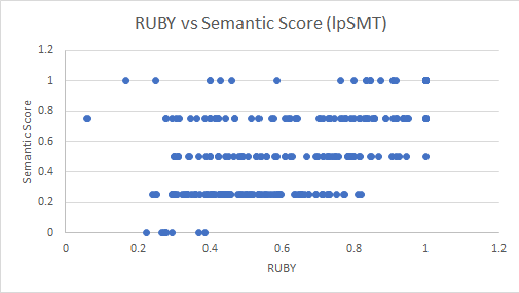
\includegraphics{img/rubyvssem_lpSMT.png}
\label{fig:RubySemlpSMT}
\end{figure}

\begin{figure}[t]
\caption{{\model} vs semantic score (mppSMT)}
\centering
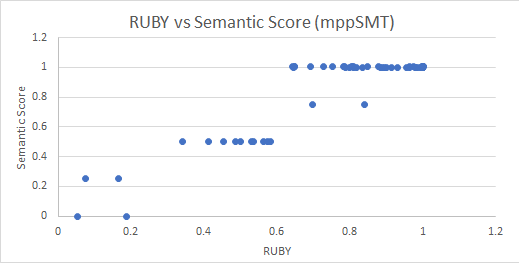
\includegraphics{img/rubyvssem_mppSMT.png}
\label{fig:RubySemMppSMT}
\end{figure}

As our experiment result, the correlation coefficients between {\model} and
semantic score are \textbf{0.764}, \textbf{0.815}, and \textbf{0.747} for the 3 models GNMT, mppSMT, and lpSMT  respectively. Comparing to the correlation of BLEU of 0.658, 0.523, and 0.570, {\model}'s results are much higher. 
In statistics, 
these values indicate a strong positive linear relationship between two 
quantitative metrics. That means one metric could be predicted by the other 
with high confidence. For example, an increase of 0.5, {\model} score can be 
interpreted as an increase of 0.4 in term of semantic score. Based on that 
information, developers can tune the SMT-based migration system in an incremental manner.

Figures~\ref{fig:RubySemlpSMT} and~\ref{fig:RubySemMppSMT} show the
scatter plots between {\model} and semantic scores on two models mppSMT
and lpSMT, respectively. For lpSMT (figure~\ref{fig:RubySemlpSMT}), 
there is a moderately strong, positive, linear association between the 
two variables with a few outliers. Beside, figure~\ref{fig:RubySemMppSMT} 
shows a strong, positive, linear association between {\model} and semantic 
score for the results translated by mppSMT. There are no outliers in the data. 
This indicates the result is consistent.

%In general, {\model} has high correlation with semantic scores. As our
%experiment result, the correlation coefficient between {\model} and
%semantic score for model mppSMT is \textbf{0.862} and for the model
%lpMSMP is \textbf{0.836}. In statistics, these values indicate a
%strong uphill linear relationship between two quantitative
%metrics. That means one metric could be predicted by the other with
%high confidence. For example, an increase of 0.5, {\model} score can
%be interpreted as an increase of 0.4 in term of Semantic score. Based
%on that information, developers can tune the system in an incremental
%manner.
%Specifically, a correlation of +0.8 implies that when 	

In general, the correlation coefficient between {\model} and semantic score cannot be 
stronger than GRS or even TRS. However, {\model} scores are available for any pair 
of the translated result and the reference code, while GRS and TRS are applicable for 
a subset of results. In our sample data, the sizes of these applicable set of methods
are quite small, for lpSMT they are \textbf{75/375} and \textbf{123/375}, and these figures
for mppSMT are \textbf{239} and \textbf{292} respectively. The summary results about correlation with semantic score is presented in \ref{fig:summary}

%While GRS is
%only computed with the migrated code with sufficient semantic
%information, {\model} does not depend on the code, even we can not parse
%PDGs and ASTs. This implies that there exist a {\model} score for any
%given code. On the other hand, in comparison with TRS, STS
%and BLEU, {\model} always outperforms the other three metrics.

	    
\subsubsection{The Use of RUBY in Comparing Models}
We conducted the same experiment on {\model} as we did with BLEU on cross models. 
Comparing models GNMT and mppSMT, we found out that in \textbf{97.7\%} of the cases, the change in {\model} score indicates the change in the same direction for Semantic score. It means an improvement in {\model} score equivalents an improvement in Semantic scores and vice versa. More interestingly, 83 of 88 cases (\textbf{94.3\%}) if a pair of translated results have the same Semantic score, they also have identical {\model} score. 
As the results showing, {\model} is a reliable metric to use in comparing different SMT-based migration models. 	

\begin{figure}
\centering
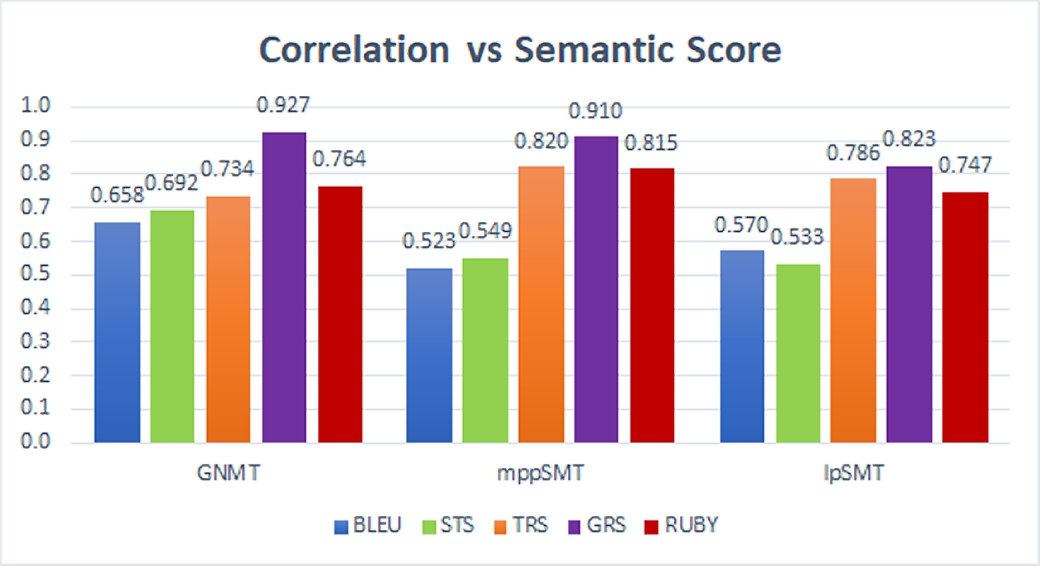
\includegraphics[scale=0.85]{img/summary.jpg}
\label{fig:summary}
\end{figure}